\documentclass[10pt, a4paper]{report}

\usepackage[utf8]{inputenc}
\usepackage[portuges]{babel}
\usepackage{blindtext}
\usepackage{enumitem}
\usepackage{cite}
\usepackage{graphicx}


\title{Projeto Programação Orientada a Objetos \\ Mestrado Integrado em Engenharia Informática}
\author{Luís Capa \\ A81960 
	\and 
	Moisés Antunes \\ A82263
	\and
	Pedro Capa \\ A83170
}
\date{\today}

\begin{document}
\maketitle
\tableofcontents

\chapter{Introdução}\label{introducao}

Neste projeto realizado no âmbito de \emph{Programação Orientada a Objetos}, foi proposto a criação de uma aplicação, identica ao \emph{e-fatura}, que permitia aos contibuintes aceder às suas faturas e às empresas aceder às faturas que inseriam no sistema, bem como calcular o valor deduzido das faturas. A aplicação tinha de fornecer diversos mecanismos para que o utilizador tivesse acesso a toda a informação relativa a este.

\chapter{Arquitetura de classes}\label{Arquitetura}

Para representar os vários intervenientes do sistema foi criado uma classe abstrata, \ref{entidades}, as despesas do sistema são representadas pelas classes \ref{Fatura} e pela \ref{FatEmpresa}. A classe \ref{Sistema} continha as principais estruturas de dados que armazenavam toda a informação.

\begin{figure}[h]
\caption{Arquitetura das classes bluej}
\centering
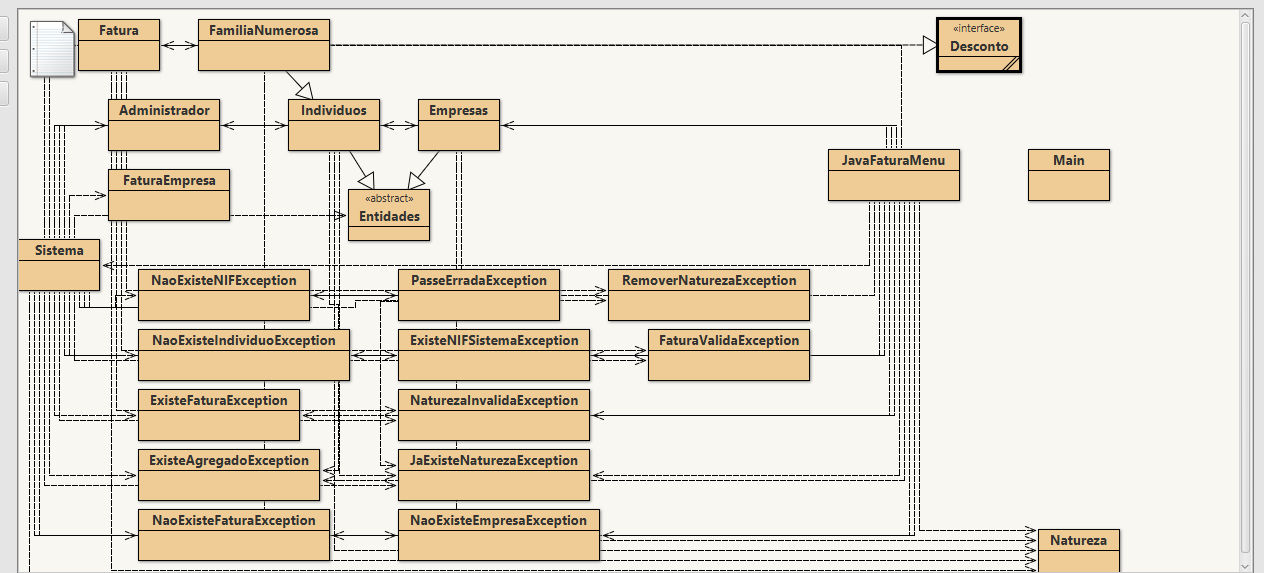
\includegraphics{classes}
\label{menu0}
\end{figure}

\section{Entidades}\label{entidades}

Esta classe foi criada com o objetivo de reduzir a repetição de código, existem vários dados comuns entre as classes \ref{Individuo} e \ref{Empresa}. Como esta classe foi criada com o objetivo de que outras classes herdem os seus métodos e variáveis de instância, então foi criada como uma classe abstrata.
A classe, tem as seguintes variáveis de instância:
\begin{itemize}
	\item NIF
	\item Nome
	\item Morada
	\item Email
	\item Password
\end{itemize}
Esta classe não continha coleções, apenas tipos de dados primitivos à exceção de Strings.

\section{Individuo}\label{Individuo}

A classe \emph{Individuo} representa os contribuintes individuais, que neste sistema só tem despesas, é uma subclasse de \ref{entidades}, logo vai herdar as variáveis de instância desta classe. As variáveis de instância desta classe são:
\begin{itemize}
	\item Dedução Fiscal
	\item Número do agregado
	\item Set com o NIF do agregado
	\item Set com as atividades que pode deduzir
\end{itemize}

\section{Empresa}\label{Empresa}

A classe \emph{Empresa} representa as entidades que fornecem serviços e que tem o poder de passar faturas, tal como a classe \ref{Individuo}, é uma subclasse de \ref{entidades}. As variáveis de instância desta classe, além das herdadas de \ref{entidades}, são:
\begin{itemize}
	\item Set de Atividades
	\item Dedução Fiscal
\end{itemize}

\section{Natureza}\label{Nat}

A classe \emph{Natureza}, era usada para indicar as atividades económicas de uma empresa e as categorias de uma fatura.
As variáveis de instância desta classe são:

\begin{itemize}
	\item Tipo
	\item Limite
	\item Dedução 
\end{itemize}

\section{Fatura}\label{Fatura}

A classe \emph{Fatura} era um documento que continha informações acerca de uma despesa de um contribuinte. As faturas, no sistema, eram apenas associadas a um individuo. Para cada fatura no sistema havia uma \emph{FatEmpresa}, que continham a Identificação da fatura e o NIF do cliente, mas cada \emph{FaturaEmpresa} era associada a uma empresa. O que destacava uma fatura era o seguinte:

\begin{itemize}
	\item Identificação
	\item NIF do emitente
	\item NIF do cliente
	\item Descrição da compra
	\item Descrição do emissor
	\item Valor da fatura
	\item Set de Naturezas
	\item Histórico da Fatura
\end{itemize}

\section{FaturaEmpresa}\label{FatEmpresa}

A classe \emph{FaturaEmpresa} era parte de uma fatura, mas estas eram associadas às empresas. Como o NIF e a Identificação de uma fatura nunca mudavam, então foi criada uma classe, para que as empresas pudessem aceder à informação total de uma fatura. Esta classe continha:

\begin{itemize}
	\item Identificação da fatura associada
	\item NIF do cliente
\end{itemize}

\section{Administrador}\label{Admin}

O \emph{Administrador} é o responsável pela aplicação e tem acesso a algumas estatísticas do sistema. Esta classe tinha as seguintes variáveis de instância:

\begin{itemize}
	\item Nome
	\item Password
\end{itemize}

\section{Sistema}\label{Sistema}

A classe mais importante no desenvolvimento da aplicação é o sistema, uma vez que toda a informação acerca das \ref{entidades}, das \ref{Fatura} e das \ref{Nat} são guardadas nesta classe:

\begin{description}[align=left]
	\item [info] Map em que a chave era o NIF da entidade e o valor era a informação de uma entidade
	\item [sistema] Map em que a chave era o NIF de um individuo e o valor era um Set de faturas associado a esse individuo
	\item [empFaturas] Map em que a chave era o NIF de uma empresa e o valor era um Set de \ref{FatEmpresa} associado a essa empresa
	\item [natureza] List de todas as atividades económicas dedutíveis
	\item [admin] Entidade com acesso total ao sistema
\end{description}

Na fase inicial do desenvolvimento desta classe, uma fatura era tanto associada a uma empresa como a um individuo, mas para garantir o encapsulamento eram criadas cópias das faturas, isto significava que os métodos que alteravam uma fatura eram obrigados a alterar em ambas as cópias. Então foi dicidido que apenas o individuo iria ter associada a fatura com a informação total e as empresas iriam ter associadas uma \emph{FatEmpresa}, que lhes permitia na mesma ter acesso às faturas, pois a \ref{FatEmpresa} tinha informação acerca do id da fatura e do NIF do cliente. Ao implementar este sistema, foi dicidido que as empresas só podem registar faturas para contribuintes individuais, ou seja, com este sistema uma empresa nunca tem despesas.
As principais estruturas utilizadas foram \emph{Map}, tendo em vista, aceder toda a informação de um individuo ou empresa, tal como a lista de todas as faturas associadas a cada entidade, através do seu número de indentificação fiscal, NIF.
Foi dicidido que este sistema iria ter, apenas um administrador. O administrador tinha o poder de criar novas naturezas, mas também podia aceder a toda a informação sobre individuos, empresas e faturas. Ainda podia ver algumas estatísticas, como os contribuintes que mais gastaram em todo o sistema.

\chapter{Ilustração da Aplicação}

A fim de desenvolver o interface da aplicação foi criada a classe \emph{JavaFaturaMenu}, que era, basicamente criar um menu que disponiblizava ao utilizador várias opções.
Para desenvolver esta classe foram criados vários métodos que utilizavam o System.out e o System.in, para poder interagir com o utilizador.
O menu foi dividido em várias fases:

\begin{itemize}
	\item Menu Inicial
	\item Menu Individuo
	\item Menu Empresa
	\item Menu Administrador
\end{itemize}

Nem todos tinham acesso a qualquer menu, o \emph{Menu Individuo} era acedido, após um individuo se registar ou dado login.
Tal como o \emph{Menu Individuo}, o mesmo se passava no \emph{Menu Empresa}, mas este era apenas acedido por empresas.
O \emph{Menu Administrador} era restrito ao administrador do sistema.

No menu inicial era feito o login ou o registo na aplicação

\begin{figure}[h]
\caption{Menu Inicial}
\centering
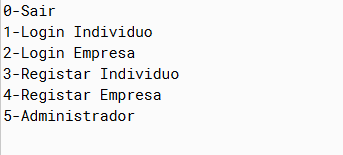
\includegraphics{Menu}
\label{menu0}
\end{figure}

Após o utilizador ter feito login ou registado como individuo, este tinha acesso ao \emph{Menu Individuo}, e eram possiblitadas as seguintes opções ao utilizador:

\begin{figure}[h]
\caption{Menu Individuo}
\centering
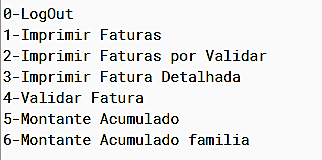
\includegraphics{Individuo}
\label{menu1}
\end{figure}

Caso fosse acedido como empresa, o utilizador tinha a possiblidade de aceder ao \emph{Menu Empresa}, e eram proporcionadas as seguintes opções:

\begin{figure}[h]
\caption{Menu Empresas}
\centering
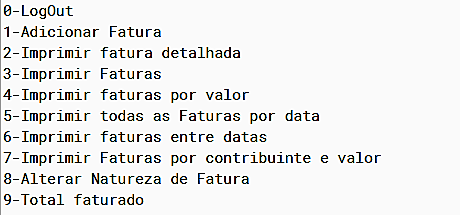
\includegraphics{Empresas}
\label{menu2}
\end{figure}

Na eventualidade do administrador aceder ao sistema, este tinha as seguintes opções:

\begin{figure}[h]
\caption{Menu Administrador}
\centering
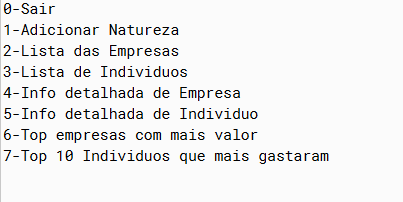
\includegraphics{Admin}
\label{menu3}
\end{figure}

Todas as alterações efetuadas pelo utilizador no sistema, só eram registadas em ficheiro, quando o utilizador saía da aplicação.

\end{document}
